\chapter{Data Analysis and Results}

\section{Introduction}
This chapter explains the data analysis and results of the research. The researcher
carefully examined the data and gave illustrations in terms of tables, percentages,
graphs and descriptive statistics.

\section{Data Preprocessing}
In this chapter, the author present the analysis of the data and the results obtained from applying the risk modeling 
techniques outlined in the methodology. Cleaning the data by removing any duplicate records, handling missing 
values, and addressing outliers.

\subsection{Descriptive analytics}
\begin{figure}[h]
    \centering
    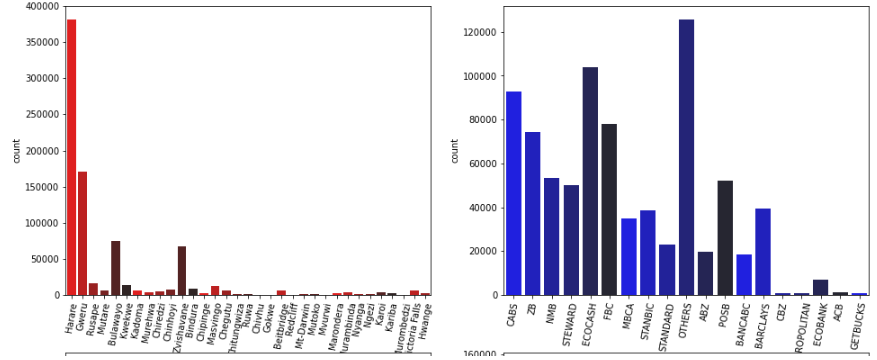
\includegraphics[width=1\linewidth]{image1}
    \caption{Data distribution 1}
    \label{fig:example}
\end{figure}
\newpage
\subsubsection{Box and Whisker Plot}
\begin{figure}[h]
    \centering
    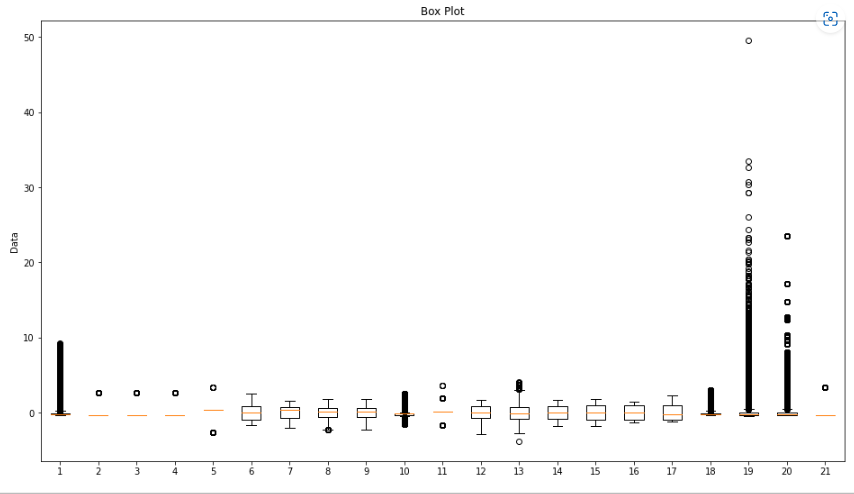
\includegraphics[width=1\linewidth]{image7}
    \caption{Box and Whisker Plot}
    \label{fig:example}
\end{figure}

\subsection{Outliers detections}
The author used the box and whisker plot to determine if there are any outliers in the data set and found out that there
were various columns with many outliers. as shown on the fig below.\\
1) orange - Fraud   2) blue - Not Fraud\\\\
\textbf{data with many otliers\\}
\begin{figure}[h]
    \centering
    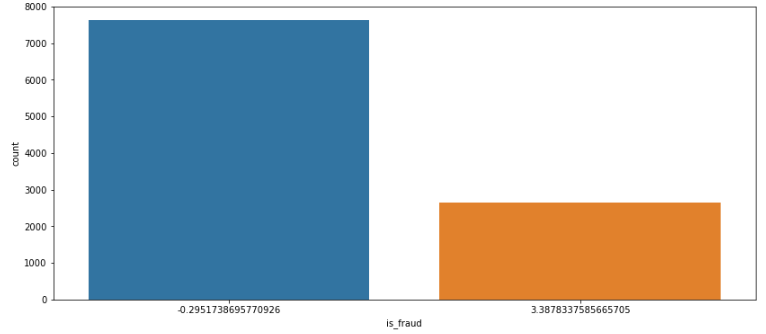
\includegraphics[width=0.7\linewidth]{image5}
    \caption{Data distribution for Outliers}
    \label{fig:example}
\end{figure}
\newpage
The author then carried out EDA to replace outliers with the average values per each column.\\\\
\textbf{data with less otliers\\}
\begin{figure}[h]
    \centering
    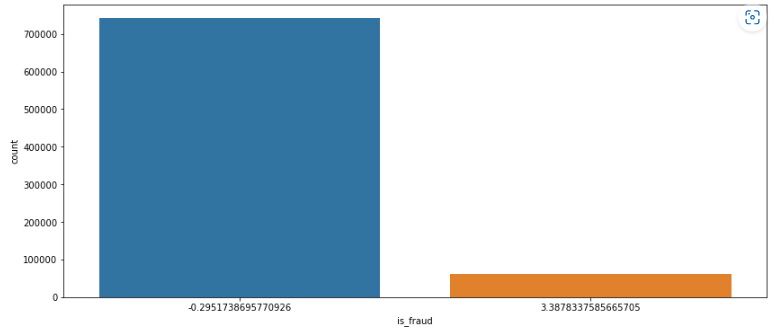
\includegraphics[width=0.7\linewidth]{image6}
    \caption{Data distribution with handled outliers}
    \label{fig:example}
\end{figure}
\subsection{Sampling}
As the researcher was dealing with a huge volume of data set of 1 200 000 rows of transactions it was necessary to 
improve the computational speed of the laptop thus data had to be sampled. The author sampled the data using the 
is\_fraud column and got the uniformly destributed data as shown below.\\
\begin{figure}[h]
    \centering
    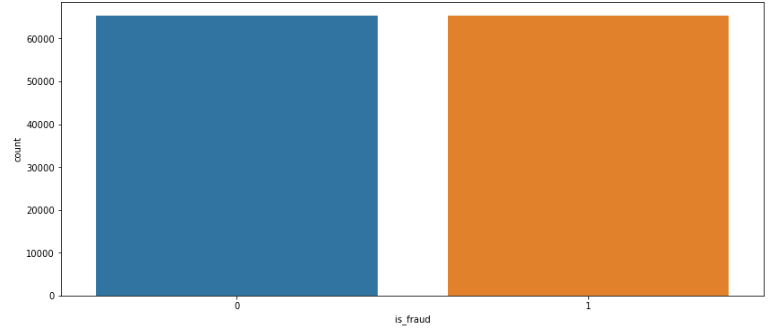
\includegraphics[width=1\linewidth]{image8}
    \caption{Uniformarly distributed data}
    \label{fig:example}
\end{figure}

\subsection{Multivariate analysis for the whole data}
\subsubsection{Correlation Diagram}
this showed that there is very weak relationship between the variables ranging from as little as from 
-0.63 to 0.0016 to 0.82\\ \\
\begin{figure}[h]
    \centering
    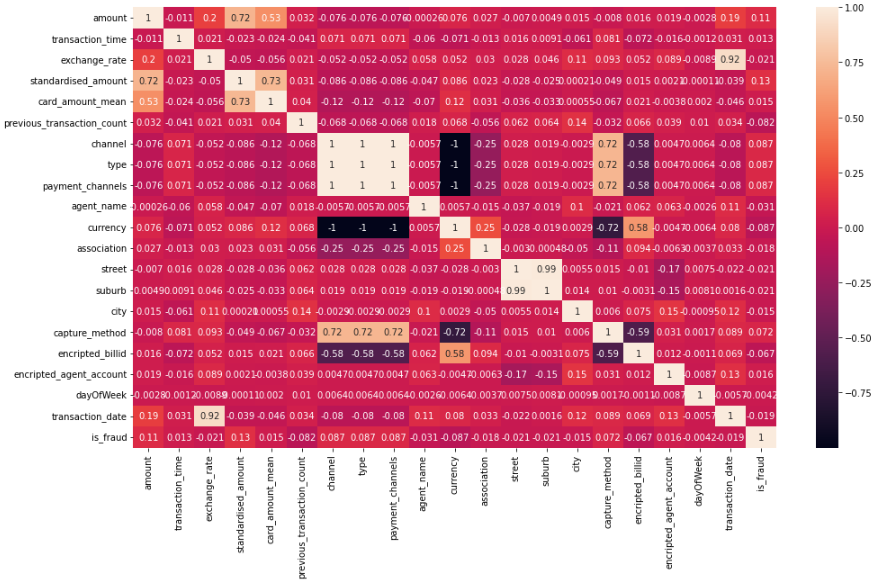
\includegraphics[width=1\linewidth]{image3}
    \caption{Correlation Graph}
    \label{fig:example}
\end{figure}
\subsubsection{Manova Table}
An F-value of -2760 is not possible and likely indicates an error in calculation or data entry.
thus further analysis had to be taken.\\
\begin{figure}[h]
    \centering
    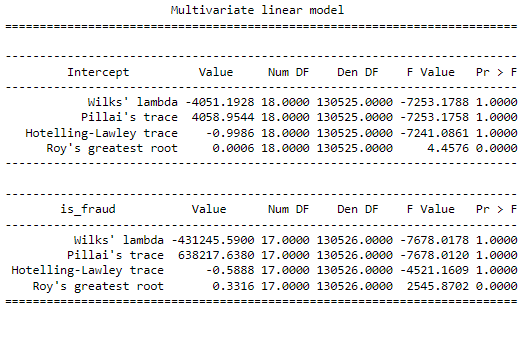
\includegraphics[width=1\linewidth]{image9}
    \caption{Manova Table}
    \label{fig:example}
\end{figure}

\section{Feature Selection and Engineering}

The author performed feature selection and engineering to identify the most relevant variables for the risk modeling 
task. Using the techniques mentioned in the methodology, assessing the correlation between variables to detect 
multicollinearity. Additionally also, used PCA to reduce the number of variables in the 
dataset while preserving the most informative features.

\subsection{Multicollinearity test}
for multicollinearity test the author used VIF.
\newpage 
\begin{table}[h]
    \centering
    \begin{tabular}{|l|l|}
      \hline
      variable & VIF \\ \hline
      amount &   2.620211\\ \hline
             transaction\_time &  24.034300\\ \hline
              exchange\_rate  & 18.169662\\ \hline
                        standardised\_amount  &  4.874732\\ \hline
             card\_amount\_mean  &  3.946724\\ \hline
   previous\_transaction\_count &   1.160809\\ \hline
                      channel    &     inf\\ \hline
                         type    &     inf\\ \hline
             payment\_channels     &    inf\\ \hline
                  agent\_name   & 3.659335\\ \hline
                   currency  & 61.099256\\ \hline
                 association  &  5.780524\\ \hline
                     street & 227.033678\\ \hline
                     suburb & 212.240119\\ \hline
                        city  &  4.013843\\ \hline
             capture\_method &  10.917950\\ \hline
           encripted\_billid  &  6.587185\\ \hline
     encripted\_agent\_account  &  4.465704\\ \hline
                   dayOfWeek  &  2.884910\\ \hline
            transaction\_date &  61.289448\\ \hline
    \end{tabular}
    \caption{Multicollinearity (VIF) table 1}
    \label{Multicollinearity (VIF) table 1}
  \end{table}
\subsubsection{Dropping varibles with range VIF greater than 10}

\newpage
\begin{table}[h]
    \centering
    \begin{tabular}{|l|l|}
        \hline
        variable & VIF \\ \hline
        transaction\_time & 11.176353\\ \hline
        standardised\_amount &  3.612614\\ \hline
        card\_amount\_mean &  3.915085\\ \hline
        previous\_transaction\_count  & 1.153174\\ \hline
        payment\_channels  & 1.964121\\ \hline
        agent\_name  & 3.335068\\ \hline
        association &  4.943633\\ \hline
        city  & 3.785845\\ \hline
        encripted\_billid &  5.154255\\ \hline
        encripted\_agent\_account &  4.000727\\ \hline
        dayOfWeek  & 2.771355\\ \hline
    \end{tabular}
    \caption{Multicollinearity (VIF) table 2}
    \label{Multicollinearity (VIF) table 2}
\end{table}

\subsection{Feature selection}
\vspace{1cm}
\begin{table}[h]
    \centering
    \begin{tabular}{|l|l|}
        \hline
        \textbf{Pearson Feature selection} & \textbf{Chi-Square Feature selection} \\ \hline
        city & city\\ \hline
        card amount mean &  encripted agent account\\ \hline
        association &  association\\ \hline
        agent name  & agent name\\ \hline
        encripted billid  & encripted billid\\ \hline
        payment channels  & payment channels\\ \hline
        standadised amount &  standadised amount\\ \hline
        previous transactions count  & previous transactions count\\ \hline
    \end{tabular}
    \caption{Feature selection table}
    \label{Feature selection table}
\end{table}
\subsection{Selected Features}
\subsubsection{Corelation between features}
\newpage
\begin{figure}[h]
    \centering
    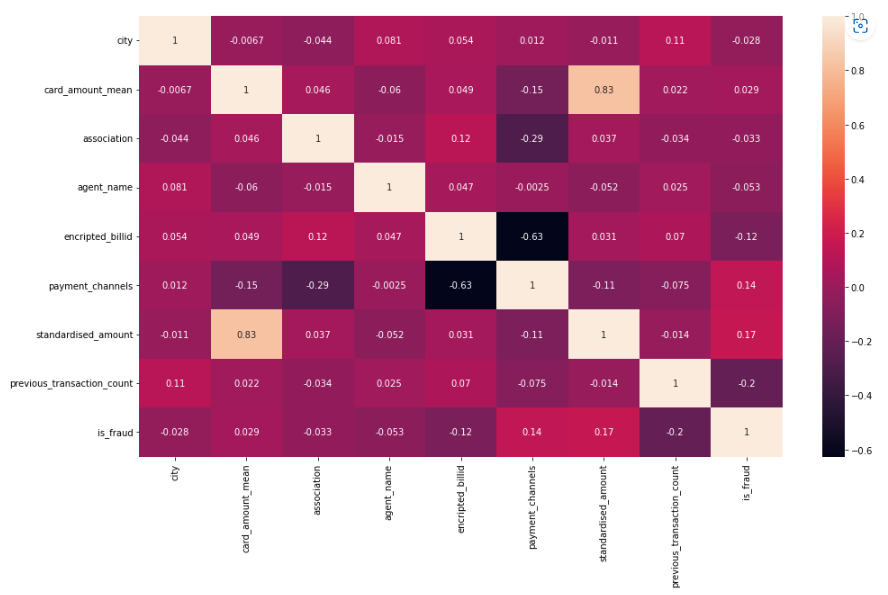
\includegraphics[width=0.9\linewidth]{image13}
    \caption{Selected Features}
    \label{fig:Selected Features}
\end{figure}
\subsubsection{Multivariate analysis between selected Features}
\vspace{1cm}
\begin{figure}[h]
    \centering
    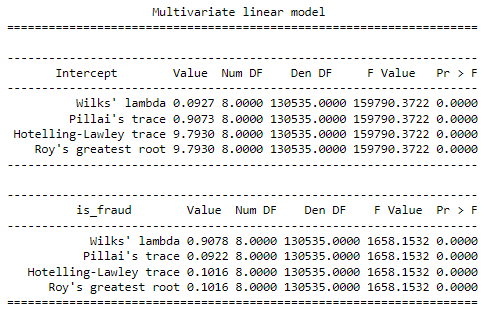
\includegraphics[width=0.7\linewidth]{image14}
    \caption{Multivariate analysis between selected Features}
    \label{fig:Multivariate analysis between selected Features}
\end{figure}
\newpage
\section{Model Training and Evaluation}
After preprocessing the data, the author moved on to training and evaluating the machine learning models.
The author employed K-Nearest Neighbors (KNN), Guasian NB, SVM, Logistic 
Regression, and XGBoost models.\\\\
For each model the dataset was split into training and testing sets using a stratified sampling approach using (70\% to 30\% ).

\subsection{Logistic Regression Model}
\vspace{1cm}
\begin{figure}[h]
    \centering
    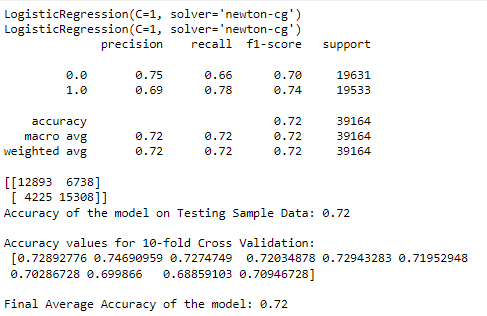
\includegraphics[width=0.8\linewidth]{image15}
    \caption{Logistic Regression Model}
    \label{fig:Logistic Regression Model}
\end{figure}
\newpage
\subsection{XG Boost Model}
\vspace{1cm}
\begin{figure}[h]
    \centering
    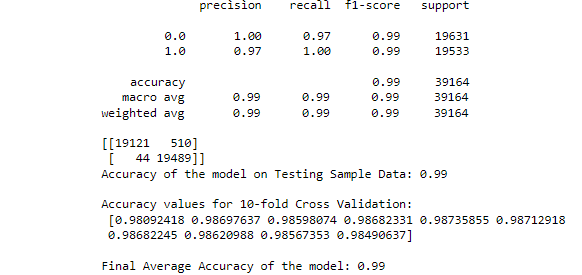
\includegraphics[width=0.8\linewidth]{image16}
    \caption{XG Boost Model}
    \label{fig:XG Boost Model}
\end{figure}
\subsection{K-nearest neighbors Model}
\vspace{1cm}
\begin{figure}[h]
    \centering
    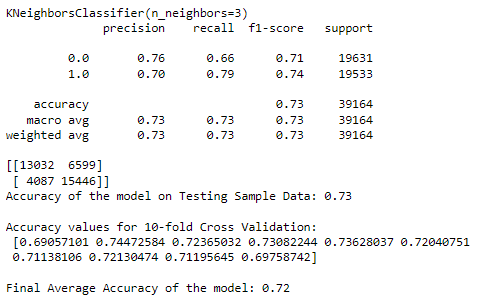
\includegraphics[width=0.8\linewidth]{image17}
    \caption{K-nearest neighbors Model}
    \label{fig:K-nearest neighbors Model}
\end{figure}
\newpage
\subsection{Guasian Naive Bayes Model}
\vspace{0.5cm}
\begin{figure}[h]
    \centering
    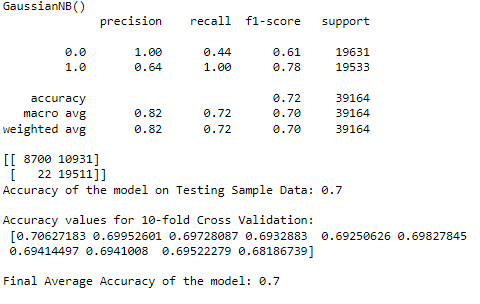
\includegraphics[width=0.6\linewidth]{image18}
    \caption{Guasian Naive Bayes Model}
    \label{fig:Guasian Naive Bayes Model}
\end{figure}
\subsection{Support Vector Model (SVM)}
\vspace{0.5cm}
\begin{figure}[h]
    \centering
    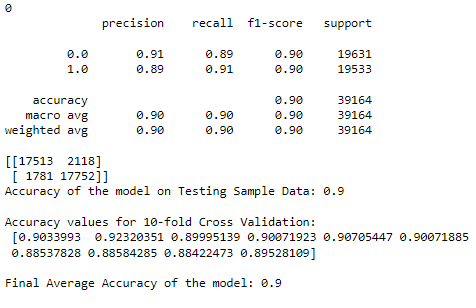
\includegraphics[width=0.6\linewidth]{image19}
    \caption{Support Vector Model (SVM)}
    \label{fig:Support Vector Model (SVM)}
\end{figure}
\section{Model Selection}
Based on results, the author performed model selection to identify the most 
suitable model for detecting fraudulent transactions in the banking sector, considered factors such as model 
performance, interpretability, and computational efficiency. Through this process, the author selected the best-performing 
model that demonstrated a balance between accuracy and computational feasibility.

\newpage
\subsection{Receiver Operating Characteristic (ROC)}
Plotting the TPR against the FPR at various discrimination thresholds. 
The TPR is the fraction of positive instances that are correctly classified, and the FPR is the fraction of 
negative instances that are incorrectly classified.

\subsubsection{For the sampled Dataset}

\begin{figure}[h]
    \centering
    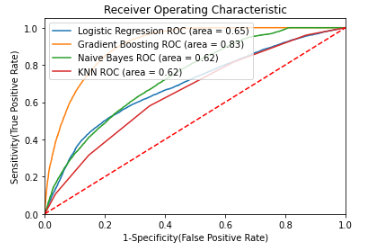
\includegraphics[width=0.7\linewidth]{image21}
    \caption{The ROC}
    \label{fig:The ROC}
\end{figure}

\subsection{Accuracy recall graphs}

\begin{figure}[h]
    \centering
    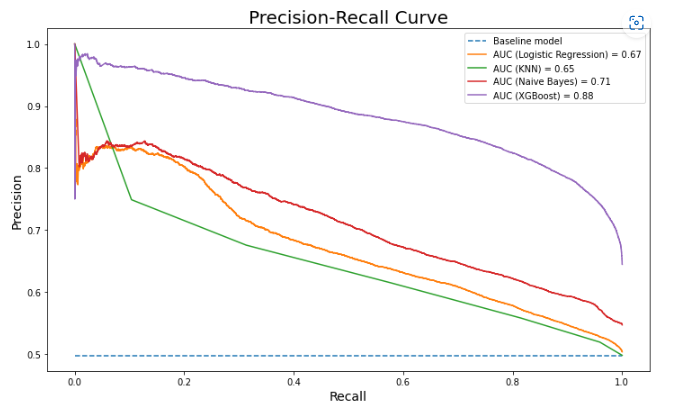
\includegraphics[width=0.7\linewidth]{image22}
    \caption{Accuracy recall graphs}
    \label{fig:Accuracy recall graphs}
\end{figure}

\section{Real-Time Predictions}
In addition to model selection, Author also implemented app for real-time predictions utilising Flask, Jupyter and 
react.js as the backend technologies to expose the machine learning models as RESTful API endpoints. This 
allowed for processing incoming transaction data in real-time and generate predictions efficiently.\\ 

\begin{figure}[h]
    \centering
    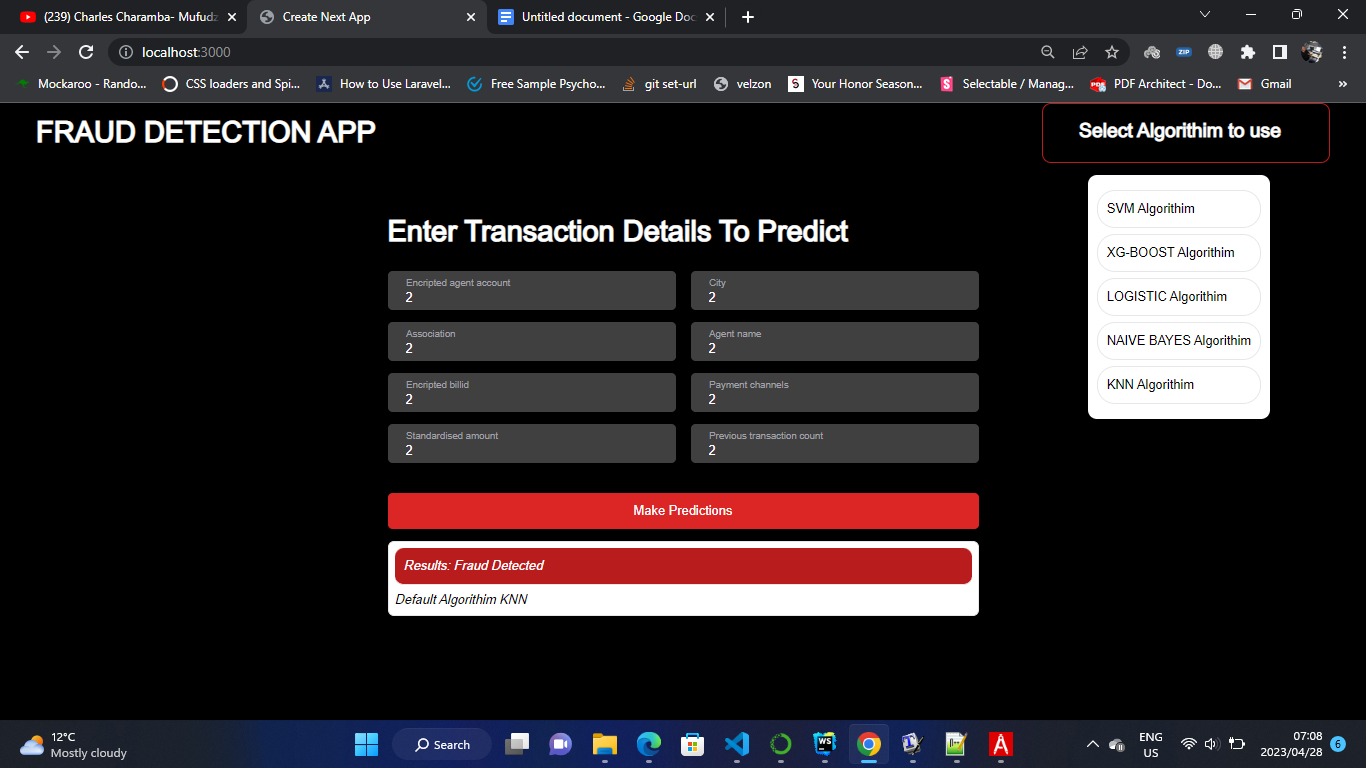
\includegraphics[width=1\linewidth]{image23}
    \caption{Web based application Interface for Real-Time Predictions}
    \label{fig:Web based application Interface for Real-Time Predictions}
\end{figure}

\section{Results and Findings}
The author presented the results and findings derived from the analysis showing performance metrics 
of each model, highlighting their accuracies, precisions, recalls, and F1 scores. Additionally, the author analyzed the 
significance of the selected features and their impact on fraud detection. The author also provided insights into the 
characteristics of fraudulent transactions identified by the models.\\\\
The best perfoming Algorithim was Support vector machine learning algorithim which had an accuracy of 90\% comparing others which were around 70\%
thus this research is in sync with the existing literature which supported SVM as the best algorithim for classification purposes.

\section{Limitations and Future Work}
The author acknowledged the limitations of his study, such as the availability of labeled data, potential biases in the 
dataset, and the scope of the models utilized. Also, the need for further research to enhance the accuracy 
and robustness of the risk modeling approach. Future work could involve incorporating additional features, 
exploring ensemble methods, or considering advanced techniques like deep learning for improved fraud detection.\\\\
In summary, this chapter presented the comprehensive analysis of the data and the results obtained from applying the 
risk modeling techniques outlined in the methodology. It provided insights into the model performance, feature 
importance, and the potential of real-time predictions. The findings contribute to the understanding and advancement 
of fraud detection in the banking sector while acknowledging the scope for further improvements and future research.

\section{Developed App and source code}

\textbf{For the data analysis code visit} \\
https://github.com/C-Maringe/my-thesis/tree/big-data-analysis \\\\
\textbf{For the Fast Api backend code visit} \\
https://github.com/C-Maringe/my-thesis-backend \\\\
\textbf{For the React.js Code visit} \\
https://github.com/C-Maringe/my-thesis \\\\
\textbf{For Real Time Predictions visit} \\
https://my-thesis-sigma.vercel.app \\\\